\chapter{OpenStack}
OpenStack è una piattaforma ideata per la realizzazione e la gestione di infrastrutture cloud complesse, pubbliche e private.
Sviluppato inizialmente da NASA e Rackspace, è oggi amministrato dalla OpenStack Foundation, rilasciato sotto licenza Apache, e sostenuto da aziende del calibro di IBM, Cisco, Citrix, Dell, Oracle e Red Hat.
E' composto da una serie di progetti che si occupano dell'amministrazione delle risorse seguendo il paradigma \textit{infrastructure-as-a-service}; fornisce quindi strumenti per gestire pool di macchine virtuali, lo storage, e le risorse di rete all'interno di un data-center cloud.
Il progetto è open-source ed è interamente realizzato utilizzando il linguaggio Python, seguendo un'architettura totalmente modulare; ogni componente è indipendente dagli altri, e può vivere anche in modalità stand-alone.
I vari produttori solitamente producono delle derivazioni della piattaforma OpenStack, che si differenziano tra loro per la metodologia di automazione del deployment dei componenti e dal parco servizi offerto.
Una di queste metodologie di automazione è rappresentata da DevStack (\textit{http://devstackurl\cite{devstackurl}}), distribuzione di OpenStack orientata allo sviluppo e al testing.
OpenStack è strutturato secondo un approccio multi-tenant, ed offre un livello di astrazione tale da riuscire a garantire molte delle proprietà di sicurezza descritte nel primo capitolo.
I sorgenti sono disponibili nel repository GitHub \textit{https://github.com/openstack/}
\paragraph{}
Nell'ambito del progetto di tesi è stato utilizzato DevStack in configurazione all-in-one\footnote{Tenendo tutti i componenti su un'unica macchina} come riferimento per implementare velocemente alcune delle proprietà di sicurezza su cui sono stati effettuati i test.
In una fase successiva è stato effettuato il deploy manuale di un'infrastruttura più complessa distribuita su cinque nodi.

\section{Componenti di OpenStack}
Tutti i componenti sono implementati come servizi, che espongono delle API REST, invocabili tramite un'interfaccia a riga di comando o la dashboard grafica Horizon.
Grazie alla struttura fortemente modulare e alla natura di software open-source, chiunque può sviluppare un proprio componente seguendo le linee guida della Open Stack Foundation.\cite{GuidelinesOpenstackHacking}
La comunità  OpenStack ha comunque identificato una serie componenti che costituiscono il nucleo dell'intera piattaforma, essi sono considerati parte integrante del progetto e vengono perciò mantenuti ufficialmente dalla comunità OpenStack.
\begin{figure}[H]
\centering
\makebox[\textwidth]{
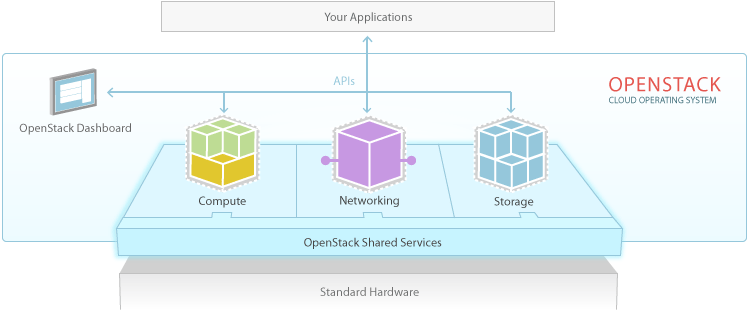
\includegraphics[width=\textwidth]{immagini/openstack-software-diagram.png}
}
\caption{Struttura della Piattaforma Openstack\cite{openstacksoftware}}\label{openstacksw}
\end{figure}
\subsection{Identity service: Keystone}
Keystone è il componente di service-catalog, che si occupa anche di fornire i servizi di gestione delle identità, dei token e delle politiche per l'uso specifico dei progetti nella famiglia OpenStack.
E' l'implementazione della Identity API, e ha funzionalità di autenticazione basata su token (authN) e meccanismi di autorizzazione di alto livello (authZ).
E' stato recentemente ristrutturato per essere espandibile e supportare meccanismi AuthN/AuthZ come oAuth, SAML, e openID.
Nella pratica, si occupa di validare le credenziali degli utenti e dei servizi, rilasciare e gestire i token di autenticazione dopo la verifica delle credenziali, e di gestire il catalogo dei servizi tenendo traccia dei relativi endpoint e i livelli di autorizzazione ad essi associati.
Supporta numerosi identity provider di back-end. L'implementazione più comune prevede l'utilizzo di MariaDB per la memorizzazione dei ruoli, delle credenziali e delle sessioni, ma è possibile strutturare architetture federate tramite LDAP o meccanismi di single-sign-on.

\subsubsection{Concetti fondamentali}

\paragraph{Utente}
Rappresentazione digitale di un utente, sistema, servizio che utilizza OpenStack.
Se è un utente ad effettuare la richiesta a Keystone (e l'autenticazione ha esito positivo), il servizio rilascia un token per effettuare le varie richieste.
Gli utenti hanno delle credenziali di login, oppure dei token per accedere alle risorse.
Possono essere direttamente assegnati ad uno o più progetti (\textit{tenant}), che costituiscono un ambiente isolato (\textit{tenant-isolation})
\paragraph{Credenziali}
Dati che confermano l'identità dell'utente (es: nome utente e password, nome utente e chiave API, token di autenticazione)
\paragraph{Autenticazione}
Processo utilizzato per confermare l'identità di un utente, in base alle credenziali fornite.
Una volta avvenuta l'autenticazione, si procede con il rilascio di un token che verrà poi utilizzato per tutte le richieste a seguire.
\paragraph{Token}
Stringa alfanumerica utilizzata per accedere alle API di OpenStack e alle risorse. Può essere revocato in qualunque momento, ed è valido per un periodo definito.
\paragraph{Progetto o tenant}
Un container utilizzato per raggruppare o isolare le risorse. I tenant isolano anche gli oggetti del servizio di identità.
A seconda delle esigenze, potrebbe corrispondere a un cliente, a un'organizzazione o a un progetto.
\paragraph{Servizio}
Un servizio di OpenStack, come Nova, Swift, Glance. Un servizio è caratterizzato da uno o più endpoint, tramite i quali gli utenti possono contattarlo per consultare le risorse da esso custodite ed eseguire le operazioni da esso consentite, nei limiti dei loro privilegi.
\paragraph{Endpoint}
Un indirizzo accessibile via rete per contattare un servizio, solitamente è un URL.
\paragraph{Ruolo}
Una personalità con un insieme definito di privilegi e diritti, su determinate operazioni.
Il token è legato alla lista dei ruoli dell'utente o servizio a cui si riferisce, cosìcche l'utente possa eseguire tutte le operazioni associate all'insieme aggregato dei ruoli a cui appartiene.

\begin{figure}[H]
\centering
\makebox[\textwidth]{
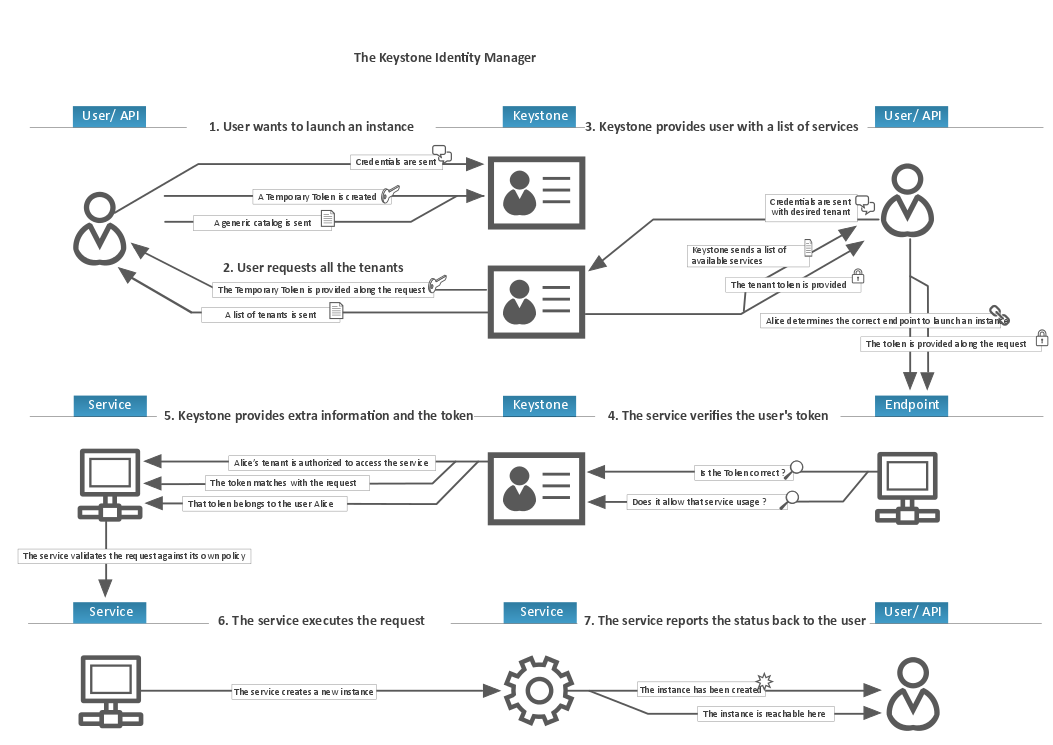
\includegraphics[width=\textwidth]{immagini/KEYSTONE.png}
}
\caption{Diagramma funzionale di Keystone\cite{openstackkeystone}}\label{openstackkeystone}
\end{figure}

\subsection{Compute service: Nova}
\subsection{Image service: Glance}
\subsection{Networking service}
\subsubsection{Nova-network}
\subsubsection{Neutron}
\subsection{Object-storage service: Swift}
\subsection{Block-storage service: Cinder}
\subsection{Orchestration service: Heat}
\subsection{Altri servizi} 
\subsubsection{Database service: Trove}
\subsubsection{Bare-metal service: Ironic}
\subsubsection{Data-processing service: Sahara}
\subsubsection{Messaging service: Zaqar}
\subsubsection{Key management service: Barbican}
\subsubsection{DNS service: Designate}
\subsubsection{Shared Filesystem service: Manila}
\subsubsection{Application catalog service: Murano}
\subsubsection{Governance service: Congress}
\subsubsection{Workflow service: Mistral}
\subsubsection{Key-value store \textit{as-a-service}: MagnetoDB}

\section{Servizi di supporto}
\subsection{Dashboard: Horizon}
\subsection{Telemetry-service: Ceilometer}
\subsection{Deployment: TripleO}
\subsection{Command-line client}
\subsection{Benchmark-service: Rally}
\section{Deploy di OpenStack con DevStack}
\subsection{Devstack e SSL}
\section{Sicurezza e certificazione di OpenStack}